% Author: Max Melching, 2025
% Inspiration: https://en.wikipedia.org/wiki/File:Kepler_laws_diagram.svg
\documentclass[border=3pt,tikz]{standalone}


\usepackage{tikz}
\usepackage{tikz-3dplot}
\usepackage[outline]{contour}
\usepackage{xcolor}

\colorlet{mydarkred}{red!55!black}
\colorlet{myred}{red!85!black}
\colorlet{mydarkorange}{orange!80!black}
\colorlet{mydarkblue}{blue!50!black}


\usetikzlibrary{3d, arrows.meta}


\tikzset{
    >={Stealth[inset=0,angle'=27]},
    mylabel/.style={
        midway,
    },
    mylabelarrow/.style={
        <->,
        thick,
    },
    orbit/.style={
        % mydarkred,
        mydarkblue,
        very thick,
    },
    innerline/.style={
        dashed,
        % mydarkblue,
    },
    foci/.style={
        fill,
        myred,
    },
    focilabel/.style={
        myred,
    },
    sun/.style={
        % line width=0,
        % fill=orange,
        orange!40!white,
        outer color=orange!40!white,
        inner color=orange,
    },
    body/.style={
        fill,
        mydarkorange,
    },
    bodylabel/.style={
        mydarkorange,
    },
    COMbody/.style={
        fill,
        teal,
    },
    COMbodylabel/.style={
        teal,
    },
}


\begin{document}


% \begin{tikzpicture}%[z={(10:10mm)},x={(-45:5mm)}]
%     \def\a{2.5}  % Semi-major axis
%     \def\eps{0.8}  % Eccentricity
%     \pgfmathsetmacro{\b}{\a*(1 - \eps^2)^.5}  % Semi-minor axis
%     \pgfmathsetmacro{\e}{\a*\eps}  % Linear eccentricity


%     % -- Ellipse stuff
%     \draw[orbit] (0,0) ellipse (\a cm and \b cm);

%     \draw[innerline] (-\a, 0) -- (\a, 0);
%     \draw[mylabelarrow, shift={(0,-1.1*\b)}] (-\a, 0) -- (0, 0) node[mylabel, below] {$a$};

%     \draw[innerline] (0, -\b) -- (0, \b);
%     \draw[mylabelarrow, shift={(1.1*\a, 0)}] (0, \b) -- (0, 0) node[mylabel, right] {$b$};


%     % -- Focal points
%     \draw[foci] (-\e, 0) circle(0.08) node[focilabel, below] {$F_1$};
%     \draw[mylabelarrow, shift={(0,-1.1*\b)}] (\e, 0) -- (0, 0) node[mylabel, below] {$e$};
%     \draw[foci] (\e, 0) circle(0.08) node[focilabel, below] {$F_2$};


%     % -- Origin
%     \coordinate (O) at (0, 0);
%     % \coordinate (O) at (-0.8*\a, 1.2*\b);
%     % \coordinate (O) at (-0.2*\a, 1.5*\b);
%     % With others math is not mathing (relative coordinate visualization not so intuitive anymore)

%     \node[below right, bodylabel] at (O) {$O$};


%     % -- Center of mass and relative coordinate
%     % \coordinate (COM) at (-\e, 0);
%     \coordinate (COM) at (-\e/2, 0);
    
%     \draw[COMbody] (COM) circle (0.07) node[above, COMbodylabel] {$M$};
%     \draw[->, thick, COMbody] (O) -- (COM) node[midway, below, COMbodylabel] {$\vec{R}$};


%     \def\relcordangle{42 + 180}
%     % \pgfmathsetmacro{\x}{\a*cos(\relcordangle)}
%     % \pgfmathsetmacro{\y}{\b*sin(\relcordangle)}
%     % \coordinate (relcoord) at (\x, \y);
%     \coordinate (relcoord) at ({\a*cos(\relcordangle)}, {\b*sin(\relcordangle)});
    
%     \draw[COMbody] (relcoord) circle (0.07) node[above, COMbodylabel] {$\mu$};
%     \draw[->, thick, COMbody] (O) -- (relcoord) node[midway, below, COMbodylabel] {$\vec{r}$};


%     % -- Component masses
%     \coordinate (m1) at ($ (COM) + 0.25*(relcoord) $);
%     \coordinate (m2) at ($ (COM) - 0.75*(relcoord) $);
%     % -- Note: the factors in front of each relcoord must sum to 1 as they represent m2/M, m1/M

%     \draw[body] (m1) circle (0.07) node[below, bodylabel] {$m_1$};
%     \draw[body] (m2) circle (0.07) node[above, bodylabel] {$m_2$};

%     \draw[->, thick, COMbody] (m2) -- (m1) node[midway, above, COMbodylabel] {$\vec{r}$};
% \end{tikzpicture}



% -- V2: Separate figures next to each other

\def\a{2.5}  % Semi-major axis
\def\eps{0.8}  % Eccentricity
\pgfmathsetmacro{\b}{\a*(1 - \eps^2)^.5}  % Semi-minor axis
\pgfmathsetmacro{\e}{\a*\eps}  % Linear eccentricity


% \begin{minipage}{0.5\textwidth}
    \begin{tikzpicture}
        % -- Origin
        \coordinate (O) at (0, 0);
        % \coordinate (O) at (-0.8*\a, 1.2*\b);
        % \coordinate (O) at (-0.2*\a, 1.5*\b);
        % With others math is not mathing (relative coordinate visualization not so intuitive anymore)

        \node[below right, bodylabel] at (O) {$O$};


        % -- Center of mass and relative coordinate
        % \coordinate (COM) at (-\e, 0);
        \coordinate (COM) at (-\e/2, 0);

        \def\relcordangle{42 + 180}
        % \pgfmathsetmacro{\x}{\a*cos(\relcordangle)}
        % \pgfmathsetmacro{\y}{\b*sin(\relcordangle)}
        % \coordinate (relcoord) at (\x, \y);
        \coordinate (relcoord) at ({\a*cos(\relcordangle)}, {\b*sin(\relcordangle)});


        % -- Component masses
        \coordinate (m1) at ($ (COM) + 0.25*(relcoord) $);
        \coordinate (m2) at ($ (COM) - 0.75*(relcoord) $);
        % -- Note: the factors in front of each relcoord must sum to 1 as they represent m2/M, m1/M

        \draw[body] (m1) circle (0.07) node[below, bodylabel] {$m_1$};
        \draw[->, thick, body] (O) -- (m1);
        \draw[body] (m2) circle (0.07) node[above, bodylabel] {$m_2$};
        \draw[->, thick, body] (O) -- (m2);

        \draw[->, thick, COMbody] (m2) -- (m1) node[midway, above, COMbodylabel] {$\vec{r}$};
        % \draw[->, thick, COMbody] (O) -- (COM) node[midway, below, COMbodylabel] {$\vec{R}$};  % Not sure about this one
    \end{tikzpicture}
% \end{minipage}%
% \begin{minipage}{0.5\textwidth}
    \begin{tikzpicture}


        % -- Ellipse stuff
        \draw[orbit] (0,0) ellipse (\a cm and \b cm);

        \draw[innerline] (-\a, 0) -- (\a, 0);
        \draw[mylabelarrow, shift={(0,-1.1*\b)}] (-\a, 0) -- (0, 0) node[mylabel, below] {$a$};

        \draw[innerline] (0, -\b) -- (0, \b);
        \draw[mylabelarrow, shift={(1.1*\a, 0)}] (0, \b) -- (0, 0) node[mylabel, right] {$b$};


        % -- Focal points
        \draw[foci] (-\e, 0) circle(0.08) node[focilabel, below] {$F_1$};
        \draw[mylabelarrow, shift={(0,-1.1*\b)}] (\e, 0) -- (0, 0) node[mylabel, below] {$e$};
        \draw[foci] (\e, 0) circle(0.08) node[focilabel, below] {$F_2$};


        % -- Origin
        \coordinate (O) at (0, 0);
        % \coordinate (O) at (-0.8*\a, 1.2*\b);
        % \coordinate (O) at (-0.2*\a, 1.5*\b);
        % With others math is not mathing (relative coordinate visualization not so intuitive anymore)

        \node[below right, bodylabel] at (O) {$O$};


        % -- Center of mass and relative coordinate
        % \coordinate (COM) at (-\e, 0);
        \coordinate (COM) at (-\e/2, 0);
        
        \draw[COMbody] (COM) circle (0.07) node[above, COMbodylabel] {$M$};
        \draw[->, thick, COMbody] (O) -- (COM) node[midway, above, COMbodylabel] {$\vec{R}$};


        \def\relcordangle{42 + 180}
        % \pgfmathsetmacro{\x}{\a*cos(\relcordangle)}
        % \pgfmathsetmacro{\y}{\b*sin(\relcordangle)}
        % \coordinate (relcoord) at (\x, \y);
        \coordinate (relcoord) at ({\a*cos(\relcordangle)}, {\b*sin(\relcordangle)});
        
        \draw[COMbody] (relcoord) circle (0.07) node[below, COMbodylabel] {$\mu$};
        \draw[->, thick, COMbody] (O) -- (relcoord) node[midway, below, COMbodylabel] {$\vec{r}$};


        % -- Component masses
        \coordinate (m1) at ($ (COM) + 0.25*(relcoord) $);
        \coordinate (m2) at ($ (COM) - 0.75*(relcoord) $);
        % -- Note: the factors in front of each relcoord must sum to 1 as they represent m2/M, m1/M

        \begin{scope}[
            opacity=0.42,
            % dotted,
            % dashed,
        ]
            \draw[body] (m1) circle (0.07) node[below, bodylabel] {$m_1$};
            \draw[body] (m2) circle (0.07) node[above, bodylabel] {$m_2$};
            
            \begin{scope}[dotted]
                \draw[->, thick, body] (O) -- (m1);
                \draw[->, thick, body] (O) -- (m2);
                
                \draw[->, thick, COMbody] (m2) -- (m1) node[midway, above, COMbodylabel] {$\vec{r}$};
            \end{scope}
        \end{scope}

    \end{tikzpicture}
% \end{minipage}



% Explanation: asymptotically, position of $\mu$ and $m_2$ are the same. This does \emph{not} mean that in this case we have $\vec{r}_2 \neq \vec{r}$, these coordinate functions can potentially differ by the constant shift $\vec{R}$ (this is not present when choose COM to be origin, i.e. in that case COM = origin and $\vec{r}_2 = \vec{r}$, which is thus a common choice). Basically, this is geometric vs coordinate statement about the ongoing mechanics.
% -> in other words, their graphs (ParametricPlot in Mathematica) would look a little different, namely precisely shifted by $\vec{R}$, but this is truly a matter of knowing how to interpret coordinate results geometrically
% -> for more general setups, this is not true anymore. See Wikipedia entry on two-body-problem, https://de.wikipedia.org/wiki/Zweik%C3%B6rperproblem. Reason: the motion on ellipse for first body is not suppressed anymore because we cannot the $m_2 / M \vec{r}$ part anymore
% -> UHHH CAREFUL; the total graphs described by $\vec{r}_2, \vec{r}$ (i.e. the curves drawn for all times in a single graph/ParametricPlot are the same), but they actually point in opposite directions due to $\vec{r}_2 = -\vec{r}$ if $\mu \approx m_2$!!!
% -> so yeah, it is truly just about solving an equivalent problem; the principle curve shape of ellipse remain the same when switching from $\vec{r}$ to $\vec{r}_2$, but positions of foci will change too (because what we do is a coordinate transformation! From CMS to Cartesian)


% -> see following two plots:


% -> ok, so here is what might be wrong: what transformation from Cartesian to COM means is that the whole thing turns into one-body problem if we choose to describe only the displacement of second body from the first, i.e. $\vec{r}$. That is because the corresponding equations are equivalent to a body of mass $\mu$ orbiting a second body of mass $M$; now, be careful with focal points: $m_1$ does lie in focal point $F_1$ in this description, which also coincides with the origin here (because this is where $\vec{r}$ starts as a vector); but the COM in this frame only lies in origin as well if m1 >> m2. When viewed from Cartesian coordinates and thus an inertial frame, both bodies undergo elliptical orbits (as both get contribution from $\vec{r}$), though with different amplitudes due to the rescaling with $m_2/M, m_1/M$, respectively; moreover, due to the addition of $\vec{R}$, we see that the focus is now shifted from origin to center of mass

% -> we perform coordinate trafo into COM and get as result that orbit of the new vector $\vec{r}$ is an ellipse (sidenote: equations look like the ones for a single particle of mass $\mu$ that orbits around); in Cartesian coordinates, this means if we place the first body in origin of coordinate system, then second body will also have elliptic orbit around it. Another interesting result from this solution (important! focal point being origin is obtained as part of the solution, not something trivial) is that focal point of the ellipse is the origin in COM, i.e. m1 in Cartesian ones. In Keplerian case, this means body 1 (which coincides with COM here) stays at rest in the origin, while second body evolves according to ellipse around first body. More generally, both bodies describe an ellipse, with semi axes determined by rescaling factors $m_2 / M, m_1 / M$, and focal point $\vec{R}$ (due to translation by this vector in the inverse transformation from COM to Cartesian)



% -- m1 >> m2 => \vec{r}_1 \approx \vec{R}
    % \begin{tikzpicture}


    %     % -- Ellipse stuff
    %     \draw[orbit] (0,0) ellipse (\a cm and \b cm);

    %     \draw[innerline] (-\a, 0) -- (\a, 0);
    %     \draw[mylabelarrow, shift={(0,-1.1*\b)}] (-\a, 0) -- (0, 0) node[mylabel, below] {$a$};

    %     \draw[innerline] (0, -\b) -- (0, \b);
    %     \draw[mylabelarrow, shift={(1.1*\a, 0)}] (0, \b) -- (0, 0) node[mylabel, right] {$b$};


    %     % -- Focal points
    %     \draw[foci] (-\e, 0) circle(0.08) node[focilabel, below] {$F_1$};
    %     \draw[mylabelarrow, shift={(0,-1.1*\b)}] (\e, 0) -- (0, 0) node[mylabel, below] {$e$};
    %     \draw[foci] (\e, 0) circle(0.08) node[focilabel, below] {$F_2$};


    %     % -- Origin
    %     \coordinate (O) at (0, 0);
    %     % \coordinate (O) at (-0.8*\a, 1.2*\b);
    %     % \coordinate (O) at (-0.2*\a, 1.5*\b);
    %     % With others math is not mathing (relative coordinate visualization not so intuitive anymore)

    %     \node[below right, bodylabel] at (O) {$O$};


    %     % -- Center of mass and relative coordinate
    %     % \coordinate (COM) at (-\e, 0);
    %     \coordinate (COM) at (-\e/2, 0);
        
    %     \draw[COMbody] (COM) circle (0.07) node[above, COMbodylabel] {$M$};
    %     \draw[->, thick, COMbody] (O) -- (COM) node[midway, above, COMbodylabel] {$\vec{R}$};


    %     \def\relcordangle{42 + 180}
    %     % \pgfmathsetmacro{\x}{\a*cos(\relcordangle)}
    %     % \pgfmathsetmacro{\y}{\b*sin(\relcordangle)}
    %     % \coordinate (relcoord) at (\x, \y);
    %     \coordinate (relcoord) at ({\a*cos(\relcordangle)}, {\b*sin(\relcordangle)});
        
    %     \draw[COMbody] (relcoord) circle (0.07) node[below, COMbodylabel] {$\mu$};
    %     \draw[->, thick, COMbody] (O) -- (relcoord) node[midway, below, COMbodylabel] {$\vec{r}$};


    %     % -- Component masses
    %     \coordinate (m1) at ($ (COM) + 0.01*(relcoord) $);
    %     \coordinate (m2) at ($ (COM) - 0.99*(relcoord) $);
    %     % -- Note: the factors in front of each relcoord must sum to 1 as they represent m2/M, m1/M

    %     \begin{scope}[
    %         opacity=0.42,
    %         % dotted,
    %         % dashed,
    %     ]
    %         \draw[body] (m1) circle (0.07) node[below, bodylabel] {$m_1$};
    %         \draw[body] (m2) circle (0.07) node[above, bodylabel] {$m_2$};
            
    %         \begin{scope}[dotted]
    %             \draw[->, thick, body] (O) -- (m1);
    %             \draw[->, thick, body] (O) -- (m2);
                
    %             \draw[->, thick, COMbody] (m2) -- (m1) node[midway, above, COMbodylabel] {$\vec{r}$};
    %         \end{scope}
    %     \end{scope}

    % \end{tikzpicture}


% -- Now m1 >> m2 AND \vec{R} = O


    % \begin{tikzpicture}


    %     % -- Ellipse stuff
    %     \draw[orbit] (0,0) ellipse (\a cm and \b cm);

    %     \draw[innerline] (-\a, 0) -- (\a, 0);
    %     \draw[mylabelarrow, shift={(0,-1.1*\b)}] (-\a, 0) -- (0, 0) node[mylabel, below] {$a$};

    %     \draw[innerline] (0, -\b) -- (0, \b);
    %     \draw[mylabelarrow, shift={(1.1*\a, 0)}] (0, \b) -- (0, 0) node[mylabel, right] {$b$};


    %     % -- Focal points
    %     \draw[foci] (-\e, 0) circle(0.08) node[focilabel, below] {$F_1$};
    %     \draw[mylabelarrow, shift={(0,-1.1*\b)}] (\e, 0) -- (0, 0) node[mylabel, below] {$e$};
    %     \draw[foci] (\e, 0) circle(0.08) node[focilabel, below] {$F_2$};


    %     % -- Origin
    %     \coordinate (O) at (0, 0);
    %     % \coordinate (O) at (-0.8*\a, 1.2*\b);
    %     % \coordinate (O) at (-0.2*\a, 1.5*\b);
    %     % With others math is not mathing (relative coordinate visualization not so intuitive anymore)

    %     \node[below right, bodylabel] at (O) {$O$};


    %     % -- Center of mass and relative coordinate
    %     \coordinate (COM) at (0, 0);
        
    %     \draw[COMbody] (COM) circle (0.07) node[above, COMbodylabel] {$M$};
    %     \draw[->, thick, COMbody] (O) -- (COM) node[midway, above, COMbodylabel] {$\vec{R}$};


    %     \def\relcordangle{42 + 180}
    %     % \pgfmathsetmacro{\x}{\a*cos(\relcordangle)}
    %     % \pgfmathsetmacro{\y}{\b*sin(\relcordangle)}
    %     % \coordinate (relcoord) at (\x, \y);
    %     \coordinate (relcoord) at ({\a*cos(\relcordangle)}, {\b*sin(\relcordangle)});
        
    %     \draw[COMbody] (relcoord) circle (0.07) node[below, COMbodylabel] {$\mu$};
    %     \draw[->, thick, COMbody] (O) -- (relcoord) node[midway, below, COMbodylabel] {$\vec{r}$};


    %     % -- Component masses
    %     \coordinate (m1) at ($ (COM) + 0.01*(relcoord) $);
    %     \coordinate (m2) at ($ (COM) - 0.99*(relcoord) $);
    %     % -- Note: the factors in front of each relcoord must sum to 1 as they represent m2/M, m1/M

    %     \begin{scope}[
    %         opacity=0.42,
    %         % dotted,
    %         % dashed,
    %     ]
    %         \draw[body] (m1) circle (0.07) node[below, bodylabel] {$m_1$};
    %         \draw[body] (m2) circle (0.07) node[above, bodylabel] {$m_2$};
            
    %         \begin{scope}[dotted]
    %             \draw[->, thick, body] (O) -- (m1);
    %             \draw[->, thick, body] (O) -- (m2);
                
    %             \draw[->, thick, COMbody] (m2) -- (m1) node[midway, above, COMbodylabel] {$\vec{r}$};
    %         \end{scope}
    %     \end{scope}

    % \end{tikzpicture}











% \begin{tikzpicture}%[z={(10:10mm)},x={(-45:5mm)}]
%     % -- For orientation
%     % \draw[->] (0,0,0) -- (xyz spherical cs:radius=1);
%     % \draw[->] (0,0,0) -- (xyz spherical cs:radius=1,latitude=90);
%     % \draw[->] (0,0,0) -- (xyz spherical cs:radius=1,longitude=90);
%     \draw[->] (0,0,0) -- (1,0,0) node {$x$};
%     \draw[->] (0,0,0) -- (0,1,0) node {$y$};
%     \draw[->] (0,0,0) -- (0,0,1) node {$z$};


%     \def\a{1}  % Semi-major axis
%     \def\b{0.75}  % Semi-minor axis
%     \def\e{0.5}  % Linear eccentricity

%     \coordinate (O) at (0,0);
%     \coordinate (FOC) at (-e,0);


%     % -- Draw ellipse in some arbitrary plane in 3D
%     \begin{scope}[
%         mydarkorange,
%         plane origin={(0,0,0)},
%         plane x={(1,0,0)},
%         % plane y={(0.707,0,-0.707)},
%         plane y={(0,0,-1)},
%         canvas is plane,
%         % canvas is zy plane at x=0,
%         shift={(\e,0,0)}
%     ]
%         \draw (0,0) ellipse (\a cm and \b cm);

%         \draw[innerline] (-\a, 0) -- (\a, 0);
%         \draw[mylabelarrow, shift={(0,-1.1*\b)}] (-\a, 0) -- (0, 0) node[mylabel] {$a$};

%         \draw[innerline] (0, -\b) -- (0, \b);
%         \draw[mylabelarrow, shift={(1.1*\a, 0)}] (0, \b) -- (0, 0) node[mylabel] {$b$};

%         \draw[foci] (\e, 0) circle(0.04);
%         \draw[mylabelarrow, shift={(0,-1.1*\b)}] (\e, 0) -- (0, 0) node[mylabel] {$e$};
%         \draw[foci] (-\e, 0) circle(0.04); 
%     \end{scope}
% \end{tikzpicture}


% \tdplotsetmaincoords{70}{120}
% % \tdplotsetmaincoords{60}{25}
% -- Doesn't do anything


% % \begin{tikzpicture}%[z={(-10:5mm)},x={(45:5mm)},y={(-45:5mm)}]
% \begin{tikzpicture}[rotate around x=-90, rotate around z=-90]%, rotate around y=60]  % y just for view checking
%         \draw[->] (0,0,0) -- (1,0,0) node {$x$};
%         \draw[->] (0,0,0) -- (0,1,0) node {$y$};
%         \draw[->] (0,0,0) -- (0,0,1) node {$z$};

%     \filldraw[orange] (0,0) circle (2pt);

%     % Define the data: {name, semi-major axis (a), semi-minor axis (b), eccentricity (e), inclination (i), longitude of ascending node (Ω), argument of periapsis (ω)}
%     \foreach \name/\a/\b/\e/\i/\Omega/\omega in {
%         Mercury/1.00/0.9796/0.2056/7.00/48.33/29.12,
%         Venus/1.868/1.868/0.0067/3.39/76.68/54.88,
%         Earth/2.584/2.584/0.0167/0.00/348.74/114.21,
%         Mars/3.938/3.9194/0.0934/1.85/49.58/286.50%,
%         % Jupiter/13.45/13.3501/0.0489/1.30/100.49/273.87,
%         % Saturn/24.65/24.5804/0.0565/2.49/113.64/339.39,
%         % Uranus/49.59/49.5359/0.0472/0.77/74.01/96.99,
%         % Neptune/77.70/77.6970/0.0086/1.77/131.78/265.64
%     } {
%         % Example action: Print the values (or use them in a drawing)
%         % \node at (0, -1.5*\a) {Planet: \name, Semi-major axis: \a, Semi-minor axis: \b, Inclination: \i°, Long. Ascend. Node: \Omega°, Arg. Periapsis: \omega°};
        
%         % Calculate the linear eccentricity to shift the ellipse
%         \pgfmathsetmacro{\c}{\a * \e}

%         % Example: Draw an ellipse with inclination, just for illustration
%         % \begin{scope}[rotate=\Omega]
%         %     % \begin{scope}[xslant=\i, rotate=\omega]
%         %     \begin{scope}[rotate around={\i:(0,0)}, xshift=\c cm, rotate=\omega]
%         %         \draw[thick] (0,0) ellipse [x radius=\a cm, y radius=\b cm];
%         %     \end{scope}
%         % \end{scope}


%         % \begin{scope}[rotate around =]
%         %     \begin{scope}[rotate around z=\Omega]
%         %         \draw[thick] (0,0) ellipse [x radius=\a cm, y radius=\b cm];
%         %     \end{scope}
%         % \end{scope}
%         % \begin{scope}[canvas is zx plane at y=0, rotate around z=\Omega]
%         %     \begin{scope}[canvas is yx plane at z=0, rotate around x=\i]
%         %         \begin{scope}[canvas is yz plane at x=-\c, rotate around z=\omega]
%         %             % Draw the orbit ellipse
%         %             \draw[thick] (0,0) ellipse [x radius=\a, y radius=\b];
%         %         \end{scope}
%         %     \end{scope}
%         % \end{scope}

%         \begin{scope}[canvas is xy plane at z=0]
%             \begin{scope}[xshift=-\c cm]
%                 % Draw the orbit ellipse
%                 \draw[thick] (0,0) ellipse [x radius=\a, y radius=\b];
%             \end{scope}
%         \end{scope}
%     }

% \end{tikzpicture}


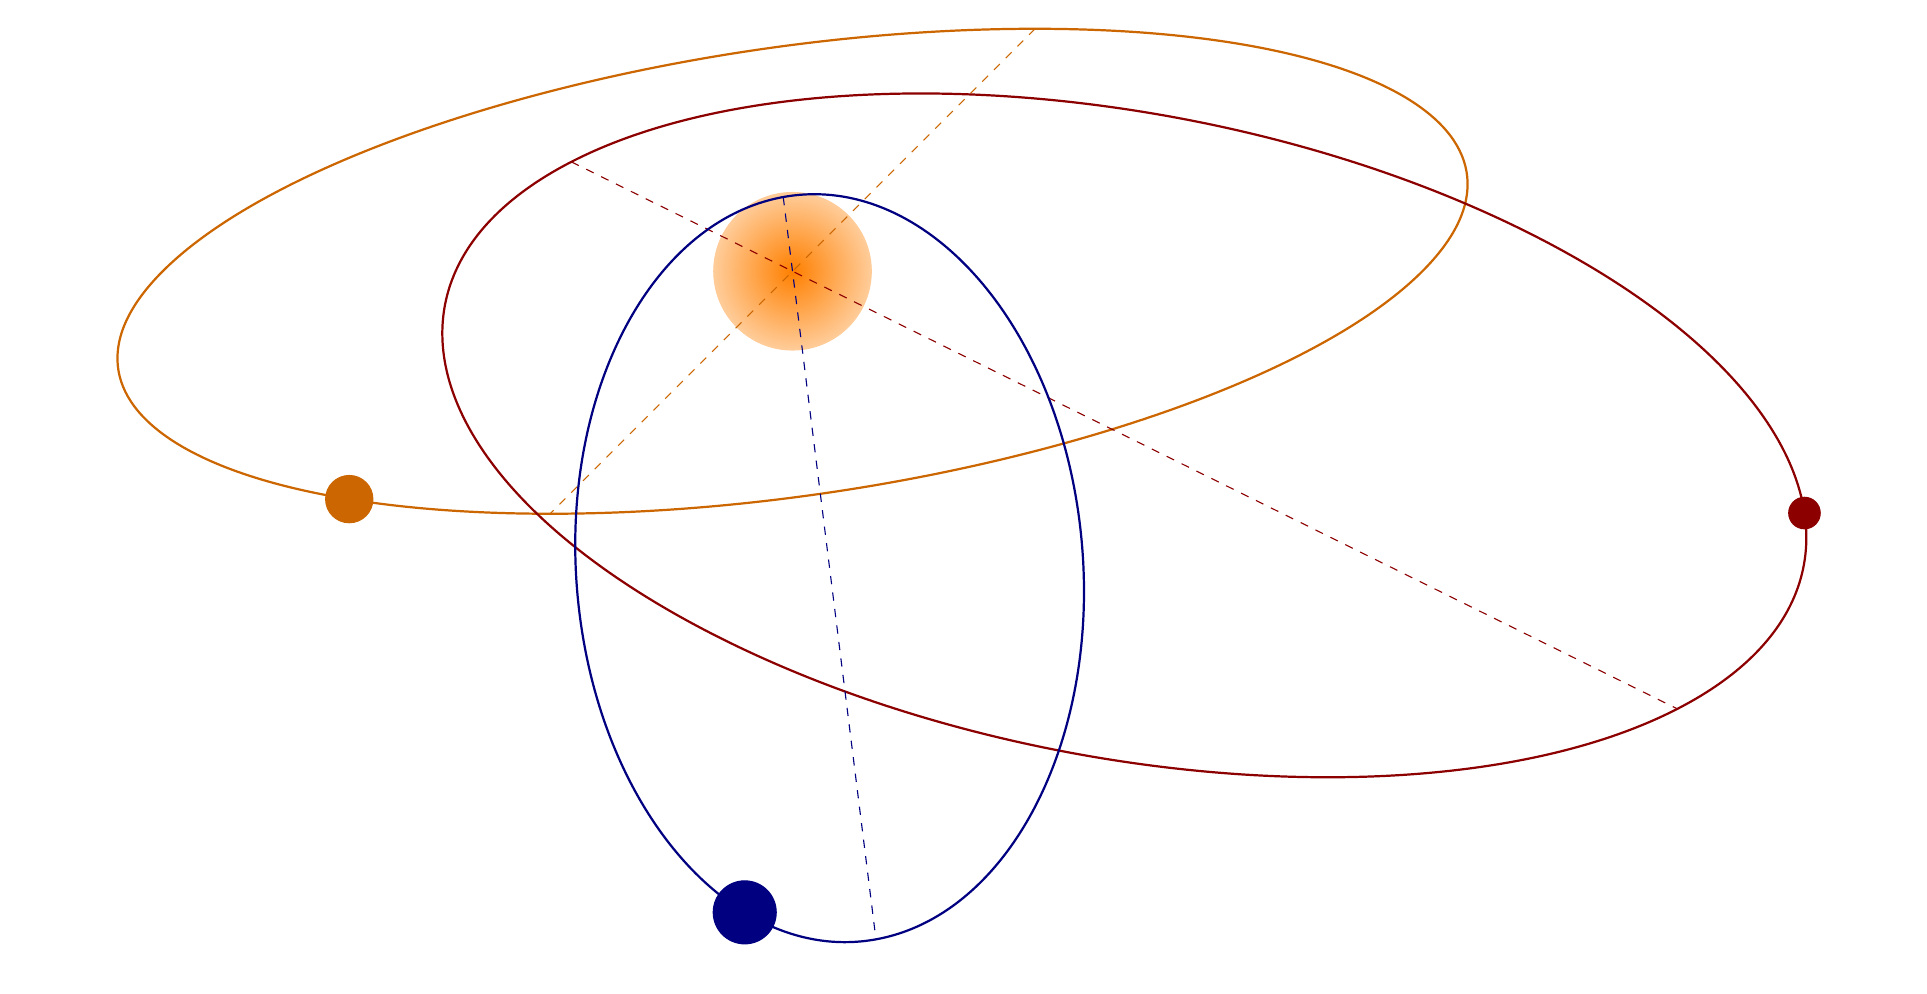
\begin{tikzpicture}[rotate around x=-90, rotate around z=-90]%, rotate around y=60]
    % \draw[->] (0,0,0) -- (1,0,0) node {$x$};
    % \draw[->] (0,0,0) -- (0,1,0) node {$y$};
    % \draw[->] (0,0,0) -- (0,0,1) node {$z$};


    \filldraw[sun] (0,0) circle (1cm);


    % \foreach \a/\b/\phi/\theta/\c in {
    %     5.0/4/0.0/0.0/mydarkorange,%
    %     8.0/3/20.0/0.0/mydarkred,%
    %     8.0/5/20.0/20.0/mydarkblue%
    % } {
    %     \pgfmathsetmacro{\e}{\a*(1 - \b^2 / \a^2)^.5}
    % \foreach \a/\eps/\phi/\theta/\c in {
    %     5.0/0/0.0/0.0/mydarkorange,%
    %     8.0/0.5/80.0/0.0/mydarkred,%
    %     4.0/0.6/30.0/45.0/mydarkblue%
    % } {
    %     \pgfmathsetmacro{\b}{\a*(1 - \eps^2)^.5}
    %     \pgfmathsetmacro{\e}{\a*\eps}


    %     \begin{scope}[
    %         rotate around z=\phi,
    %         rotate around y=\theta,
    %     ]
    %         \begin{scope}[
    %             canvas is xy plane at z=0,
    %             xshift=\e cm,
    %             \c,
    %         ]
    %             \draw[thick] (0,0) ellipse(\a cm and \b cm);

    %             \draw[innerline, \c] (-\a, 0) -- (\a, 0);
    %             \draw[innerline, \c] (0, -\b) -- (0, \b);

    %             \draw[foci] (-\e, 0) circle(0.04);
    %         \end{scope}
    %     \end{scope}
    % }
    
    \foreach \a/\eps/\incl/\longasc/\phiref/\c/\ppos/\psize in {
        8.0/0/0.0/0.0/0.0/mydarkorange/-20/0.3,%
        9.0/0.6/15.0/70.0/0.0/mydarkred/40/0.2,%
        5.0/0.8/45.0/30.0/0.0/mydarkblue/-30/0.4%
    } {
        \pgfmathsetmacro{\b}{\a*(1 - \eps^2)^.5}
        \pgfmathsetmacro{\e}{\a*\eps}


        \begin{scope}[
            rotate around z=\longasc,
        ]
            \begin{scope}[
                rotate around y=\incl,
                rotate around z=\phiref,
            ]
                \begin{scope}[
                    canvas is xy plane at z=0,
                    xshift=\e cm,
                    \c,
                ]
                    \draw[thick] (0,0) ellipse(\a cm and \b cm);

                    \draw[innerline, \c] (-\a, 0) -- (\a, 0);
                    % \draw[innerline, \c] (0, -\b) -- (0, \b);

                    % \draw[fill, \c!20!white, opacity=0.5] (0,0) ellipse(\a cm and \b cm);

                    % \draw[foci] (-\e, 0) circle(0.04);  % Verification


                    % \draw[body, \c] ({\a*cos(\ppos)}, {\b*cos(\ppos)}) circle(\psize cm);  % Circle gets rotated, too, not intended
                    % \coordinate (planet) at ({\a*cos(\ppos) cm}, {\b*sin(\ppos) cm});
                    
                    \pgfmathsetmacro{\x}{\a*cos(\ppos)}
                    \pgfmathsetmacro{\y}{\b*sin(\ppos)}
                    \coordinate (planet) at (\x cm, \y cm);
                \end{scope}
            \end{scope}
        \end{scope}

        \draw[body, \c] (planet) circle(\psize cm);
        % \draw[\c] (0, 0) -- (planet);  % For debugging
    }

    % \filldraw[sun] (0,0) circle (1cm);  % In case ellipses are filled out

\end{tikzpicture}


\end{document}